\documentclass[11pt]{article}
\usepackage[margin=1in]{geometry}
\usepackage{amsmath,amssymb,amsthm,bm}
\usepackage{booktabs,array}
\usepackage[most]{tcolorbox}
\usepackage{graphicx}
\usepackage{hyperref}
\usepackage{xcolor}
\hypersetup{colorlinks=true,linkcolor=blue!50!black,citecolor=blue!50!black,urlcolor=blue!50!black}

% ---- three-level boxes (same scheme as teaching_docs/direct_and_indirect_cartpole.tex)
\newtcolorbox{eli}{colback=green!5,colframe=green!45!black,title=ELI5,fonttitle=\bfseries,breakable}
\newtcolorbox{intu}{colback=blue!4,colframe=blue!45!black,title=Intuition,fonttitle=\bfseries,breakable}
\newtcolorbox{rig}{colback=gray!6,colframe=black!70,title=Rigor,fonttitle=\bfseries,breakable}
\newtcolorbox{warn}{colback=orange!6,colframe=orange!70!black,title=Where it breaks / what is assumed,fonttitle=\bfseries,breakable}
\newtcolorbox{expt}[1]{colback=yellow!6,colframe=yellow!50!black,title={Experiment #1},fonttitle=\bfseries,breakable}
\newtcolorbox{chk}{colback=white,colframe=green!45!black,title=Checkpoint,fonttitle=\bfseries,breakable}

\newcommand{\file}[1]{\texttt{#1}}
\newcommand{\dd}{\mathrm{d}}
\newtheorem{theorem}{Theorem}

\title{Seeing a Conjugate Point\\
\large A guided tour of the second-order theory of the calculus of variations,\\ with an interactive explorer}
\author{M.~Casey \quad (Coorbital, \file{optimal\_control\_examples/conjugate\_points/})}
\date{2026-09-24}

\begin{document}
\maketitle

\begin{abstract}
An extremal of a variational problem --- a solution of the Euler--Lagrange
equation --- is only a \emph{candidate} for a minimum. Whether it really is one
is decided by the second variation, and the second variation is decided, almost
entirely, by one geometric event: whether the extremals that leave the starting
point alongside ours come back and meet it again before the end of the interval.
The first such meeting point is the \emph{conjugate point}.

This guide builds that idea in three layers (a picture, the reasoning, the
equations) and then hands you an interactive explorer,
\file{conjugate\_point\_explorer.m}, in which you type a Lagrangian and
\emph{watch} it happen. Four independent views of the same fact appear side by
side: neighbouring extremals crossing, the zero of the Jacobi field, the slope of
the shooting function, and a negative eigenvalue of the second variation --- with
the cost $J$ actually going down along the direction that eigenvalue points to.
Every number quoted in the experiments was computed by
\file{conjugate\_point\_study.m} and is checked there against a closed form or a
second, independent instrument.
\end{abstract}

\tableofcontents

% =======================================================================
\section{What you will see}

\begin{figure}[h]
\centering
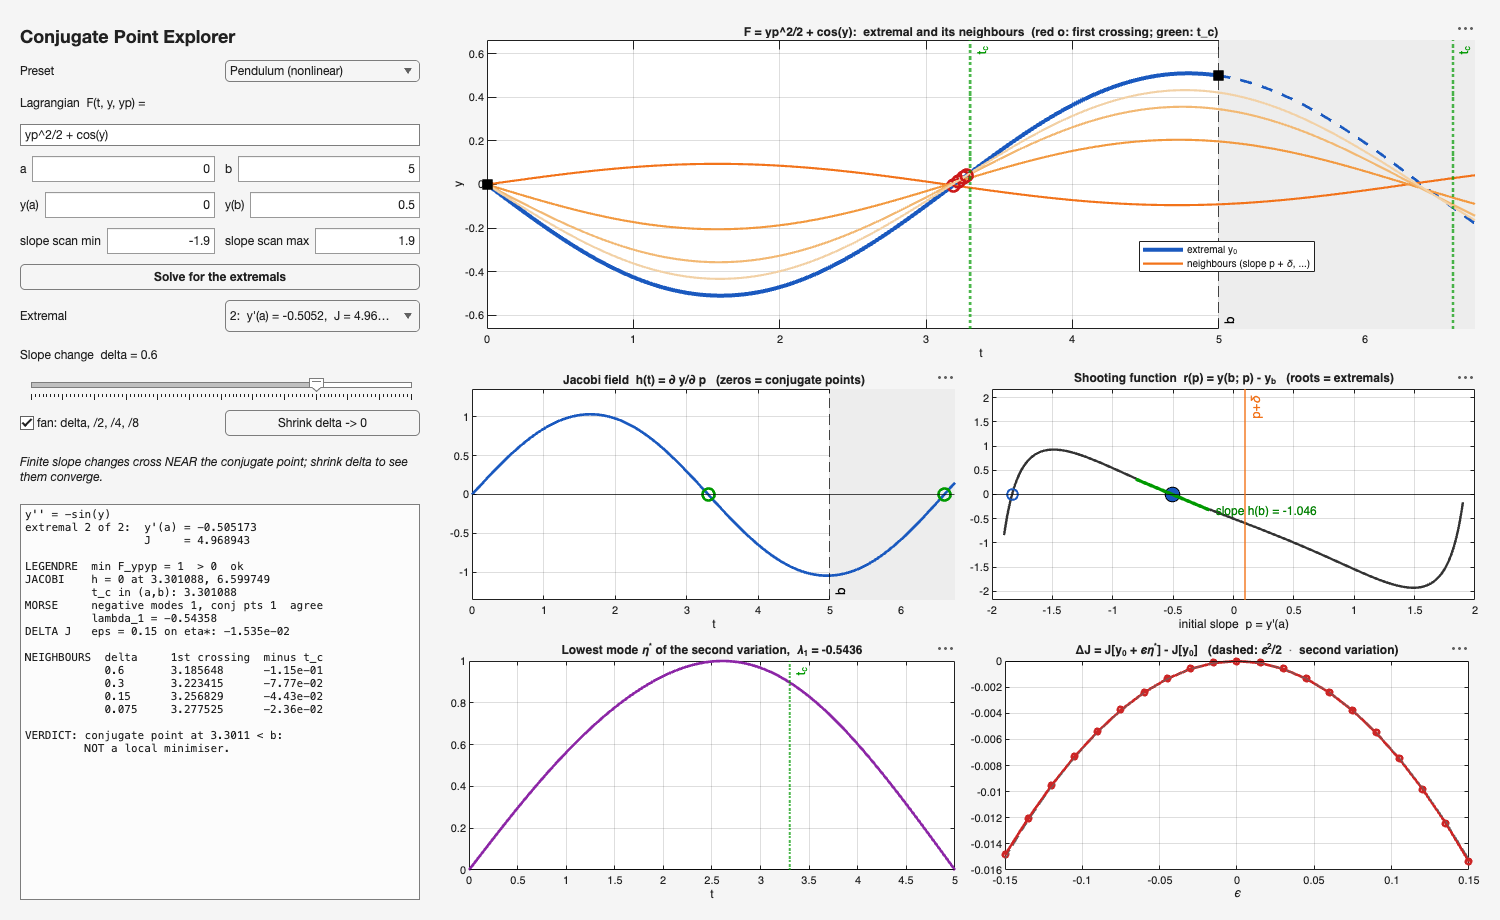
\includegraphics[width=\textwidth]{figures/explorer_pendulum.png}
\caption{The explorer on the pendulum preset. Top: the extremal (blue) and four
neighbours leaving the same start point with slightly different slopes (orange);
they cross the extremal near $t_c$ (green), well before $b = 5$. Middle: the
Jacobi field (left) and the shooting function (right). Bottom: the lowest mode of
the second variation (left), and the cost change along it (right) --- a downward
parabola, so this extremal is \emph{not} a minimiser.}
\label{fig:explorer}
\end{figure}

Run \file{conjugate\_point\_explorer} from the folder. Pick a preset or type your
own $F(t, y, y')$ (write $y'$ as \file{yp}), the interval $[a,b]$ and the end
values, and press \emph{Solve}. The explorer finds \emph{every} extremal in the
slope range you give it, and for the one you select it draws the five panels of
Figure~\ref{fig:explorer} and writes a readout with a verdict. The slider changes
the slope perturbation $\delta$; \emph{Shrink} animates $\delta \to 0$.

% =======================================================================
\section{The problem, and why an extremal is only a candidate}

\begin{eli}
You want the cheapest path from one point to another, where ``cheap'' is measured
along the whole path. The Euler--Lagrange equation finds paths where no
\emph{tiny} nudge changes the cost at first glance --- the bottom of a valley,
but also a mountain pass, or the top of a hill. To know which one you are
standing on, you have to look at how the cost \emph{curves} as you move away.
\end{eli}

\begin{rig}
The simplest problem of the calculus of variations:
\[
  \text{minimise}\quad J[y] = \int_a^b F\big(t, y(t), y'(t)\big)\,\dd t,
  \qquad y(a) = y_a,\quad y(b) = y_b .
\]
For $y = y_0 + \varepsilon\eta$ with $\eta(a) = \eta(b) = 0$,
\[
  J[y_0 + \varepsilon\eta] = J[y_0] + \varepsilon\,\delta J[\eta]
     + \tfrac{\varepsilon^2}{2}\,\delta^2 J[\eta] + O(\varepsilon^3).
\]
$\delta J = 0$ for all $\eta$ gives the Euler--Lagrange equation
$\frac{\dd}{\dd t}F_{y'} = F_y$; its solutions are \emph{extremals}. Expanded and
solved for $y''$ (this is what \file{cov\_problem.m} does symbolically),
\[
  y'' = g(t, y, y') = \frac{F_y - F_{y't} - F_{y'y}\,y'}{F_{y'y'}},
\]
which needs $F_{y'y'} \neq 0$. The second variation is
\[
  \delta^2 J[\eta] = \int_a^b \big( P\,\eta'^2 + 2R\,\eta\eta' + Q_0\,\eta^2 \big)\,\dd t,
  \qquad P = F_{y'y'},\; R = F_{y'y},\; Q_0 = F_{yy},
\]
all evaluated along $y_0$. Integrating the middle term by parts
($2R\eta\eta' = R\,(\eta^2)'$, and $\eta$ vanishes at both ends) gives the form
used in the theory,
\[
  \delta^2 J[\eta] = \int_a^b \big( P\,\eta'^2 + Q\,\eta^2 \big)\,\dd t,
  \qquad Q = F_{yy} - \tfrac{\dd}{\dd t}F_{yy'} .
\]
A minimum needs $\delta^2 J \ge 0$ for every admissible $\eta$.
\end{rig}

\begin{intu}
The $\eta'^2$ term dominates for fast wiggles: a variation that oscillates
rapidly has a huge derivative and a small amplitude. So if $P < 0$ anywhere,
wiggling there drives $\delta^2 J$ negative and the extremal is not a minimum.
That is \textbf{Legendre's necessary condition}, $P = F_{y'y'} \ge 0$. But
$P > 0$ is not enough: slow, long variations feel $Q$, and if $Q$ is negative
over a long enough stretch it can win. \emph{How long is long enough} is exactly
the question the conjugate point answers.
\end{intu}

% =======================================================================
\section{Neighbours, the Jacobi field, and the conjugate point}

\begin{eli}
Throw a ball, then throw a second one from the same spot at a very slightly
steeper angle. The two paths separate --- and on some problems they come back
together later. Where they meet again is special: from there on, there are two
nearly equal ways to have got there, and the original path stops being the best.
\end{eli}

\begin{rig}
Let $y(t;p)$ be the extremal with $y(a) = y_a$, $y'(a) = p$. Differentiate the
Euler--Lagrange equation with respect to $p$ and put $h = \partial y/\partial p$:
\[
  \frac{\dd}{\dd t}\big( R\,h + P\,h' \big) - \big( Q_0\,h + R\,h' \big) = 0
  \;\;\Longrightarrow\;\;
  \frac{\dd}{\dd t}\big( P\,h' \big) - Q\,h = 0,
  \qquad h(a) = 0,\; h'(a) = 1 .
\]
This is the \textbf{Jacobi equation}. It is the Euler--Lagrange equation of the
quadratic functional $\delta^2 J$ itself (the ``accessory problem''), and it is the
linearisation of $y'' = g$: $h'' = g_y h + g_{y'} h'$, which is the form
\file{cov\_shoot.m} integrates alongside the extremal.

A point $c \in (a, b]$ is \textbf{conjugate to $a$} if $h(c) = 0$.
\end{rig}

\begin{intu}
The neighbour with slope $p + \delta$ is
\[
  y(t; p + \delta) = y_0(t) + \delta\,h(t) + O(\delta^2).
\]
So where $h$ has a zero, the neighbour --- to first order --- is back on the
extremal. The neighbours \emph{refocus}. On a linear problem (a quadratic $F$) the
$O(\delta^2)$ term is zero and every neighbour crosses at exactly the conjugate
point, whatever $\delta$ (Figure~\ref{fig:osc}). On a nonlinear problem a finite
$\delta$ crosses \emph{near} it, and the crossing converges to $t_c$ as
$\delta \to 0$ (Section~\ref{sec:finite}).
\end{intu}

\begin{figure}[h]
\centering
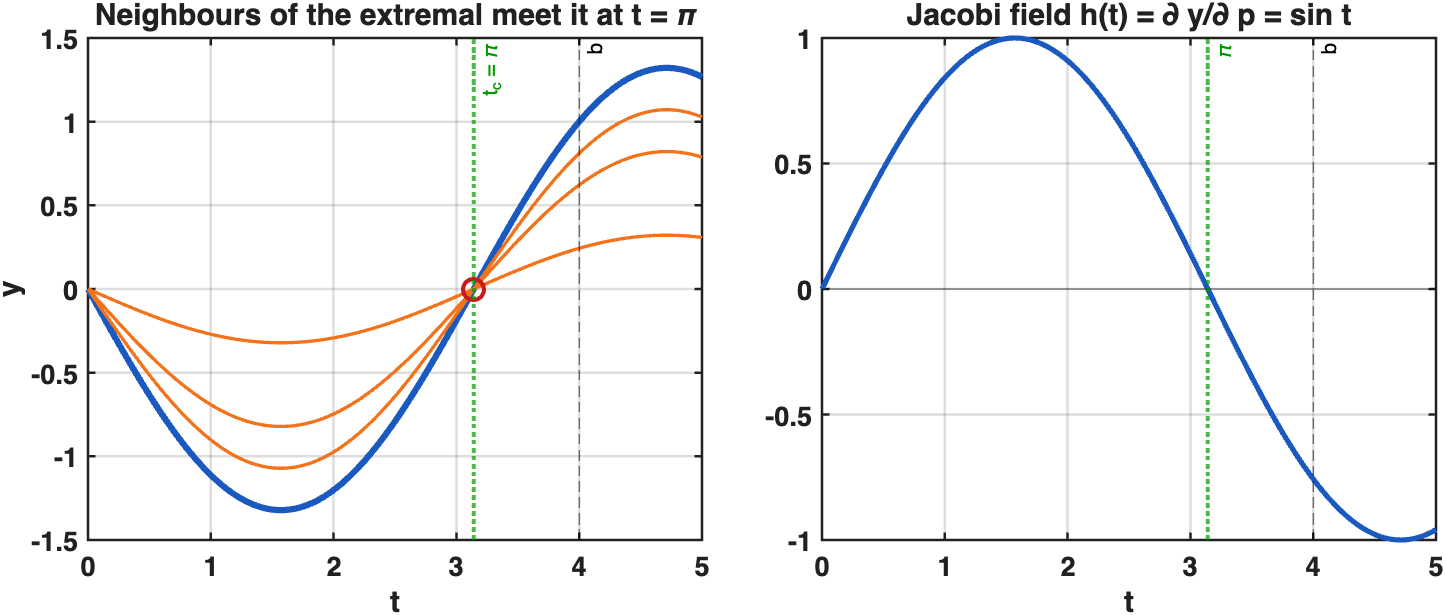
\includegraphics[width=\textwidth]{figures/oscillator_fan.png}
\caption{$F = y'^2 - y^2$ on $[0, 4]$: the extremal $y_0 = \sin t/\sin 4$ and its
neighbours with $\delta = 1, 0.5, 0.25$ all pass through $(\pi, 0)$, because the
Jacobi field is $h = \sin t$ (right). $\pi < b = 4$: not a minimiser.}
\label{fig:osc}
\end{figure}

% =======================================================================
\section{The theorem}

\begin{theorem}[Jacobi; see \cite{gelfand,liberzon}]
Let $y_0$ be an extremal with $P = F_{y'y'} > 0$ on $[a,b]$.
\begin{enumerate}
\item (Necessary) If $y_0$ is a weak local minimiser, there is no point conjugate
to $a$ in $(a, b)$.
\item (Sufficient) If there is no point conjugate to $a$ in $(a, b]$, $y_0$ is a
strict weak local minimiser.
\end{enumerate}
\end{theorem}

\begin{rig}
\textbf{Why a conjugate point inside kills the minimum.} Suppose $h(c) = 0$ with
$a < c < b$. Build the broken variation
\[
  \hat\eta(t) = \begin{cases} h(t), & a \le t \le c,\\ 0, & c < t \le b. \end{cases}
\]
It is admissible (continuous, zero at both ends) and not identically zero, and
\[
  \delta^2 J[\hat\eta] = \int_a^c \big( P h'^2 + Q h^2 \big)\,\dd t
  = \big[ P\,h\,h' \big]_a^c - \int_a^c h\big( (Ph')' - Qh \big)\,\dd t = 0,
\]
since $h(a) = h(c) = 0$ and $h$ solves the Jacobi equation. If $y_0$ were a
minimiser, $\delta^2 J \ge 0$ everywhere, so $\hat\eta$ would \emph{minimise}
$\delta^2 J$ and would have to satisfy the corner (Weierstrass--Erdmann) condition
of that problem: $P\hat\eta'$ continuous at $c$. From the right $\hat\eta' = 0$;
from the left it is $h'(c)$, so $P h'(c) = 0$, hence $h'(c) = 0$. Together with
$h(c) = 0$ that forces $h \equiv 0$ by uniqueness --- but $h'(a) = 1$.
Contradiction: $\delta^2 J$ takes negative values, and $y_0$ is not a minimum.
Rounding off $\hat\eta$'s corner produces such a negative direction explicitly.

\textbf{Counting (Morse).} More is true: the number of negative eigenvalues of
$\delta^2 J$ on variations vanishing at $a$ and $b$ equals the number of points
conjugate to $a$ in $(a, b)$ \cite{milnor}. \file{cov\_second\_variation.m}
discretises $\delta^2 J$ with finite elements and counts them --- an instrument
that never solves the Jacobi equation, so its agreement with $h$'s zeros is
genuine evidence.
\end{rig}

\begin{warn}
\begin{itemize}
\item \textbf{Weak, not strong.} The theorem compares $y_0$ with curves close in
value \emph{and} slope. Against curves that are close in value but may have very
different slopes (a strong minimum), one needs in addition the Weierstrass excess
function and a field of extremals \cite{gelfand}. The explorer tests weak
minimality only.
\item \textbf{Legendre first.} Everything assumes $P > 0$. If $P < 0$ somewhere,
Legendre's necessary condition already fails and the extremal is not a minimum
(the explorer says so and marks the Morse count as not applicable); if $P = 0$
somewhere, these tests are inconclusive.
\item \textbf{A conjugate point exactly at $b$} is the borderline case: the
second variation has a zero direction and the test is inconclusive.
\item \textbf{Numerics.} Extremals are found by scanning a slope range you
choose; an extremal outside it is not found. Zeros of $h$ are located by event
detection at \file{RelTol} $10^{-10}$; the eigenvalue count uses 300--400 finite
elements.
\end{itemize}
\end{warn}

% =======================================================================
\section{Four views of one fact}

\begin{intu}
The explorer puts four independent views of the conjugate point on screen at
once. They are computed by different code, so when they agree you are seeing the
theory, not an artefact:
\begin{enumerate}
\item \textbf{Neighbours cross.} Fly the extremal with slope $p + \delta$ and find
where it crosses $y_0$ (\file{cov\_perturbed.m}).
\item \textbf{$h$ vanishes.} Integrate the Jacobi equation and find its zeros
(\file{cov\_shoot.m}).
\item \textbf{The shooting function turns.} The extremals are the roots of
$r(p) = y(b;p) - y_b$, and $r'(p) = h(b)$. If $b$ itself is conjugate, $r'(p) = 0$
at the root: two extremals are about to merge or be born. That is a fold
(Experiment~5).
\item \textbf{The second variation goes negative.} The number of negative
eigenvalues of $\delta^2 J$ equals the number of conjugate points in $(a, b)$, and
the lowest eigenvector $\eta^*$ is a direction in which $J$ actually decreases:
$J[y_0 + \varepsilon\eta^*] - J[y_0] < 0$, computed exactly, not just predicted
(\file{cov\_second\_variation.m}).
\end{enumerate}
\end{intu}

\begin{figure}[h]
\centering
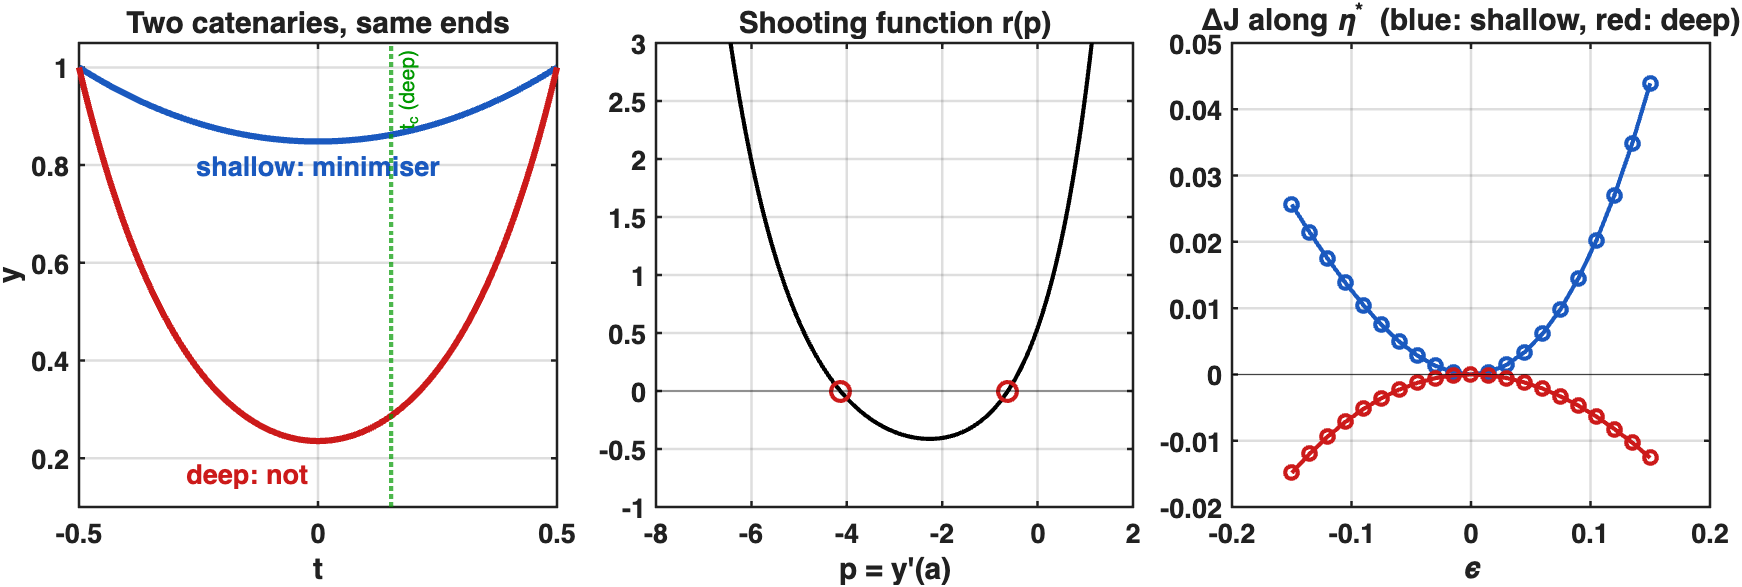
\includegraphics[width=\textwidth]{figures/catenary.png}
\caption{The minimal surface of revolution, $F = y\sqrt{1 + y'^2}$, $y(\pm\tfrac12) = 1$.
Left: two catenaries join the ends; the deep one has a conjugate point at
$t_c = 0.1529$. Middle: the shooting function has two roots, with slopes of
opposite sign ($r' = h(b)$). Right: $\Delta J$ along each extremal's lowest mode ---
up for the shallow one, down for the deep one.}
\label{fig:cat}
\end{figure}

\begin{figure}[h]
\centering
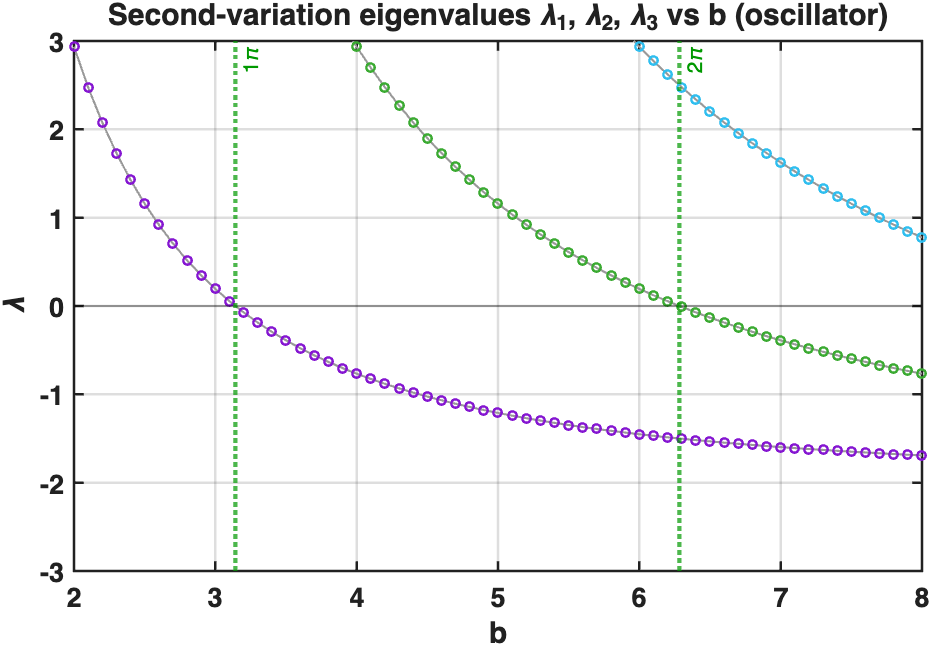
\includegraphics[width=0.62\textwidth]{figures/morse_eigenvalues.png}
\caption{The three lowest eigenvalues of the second variation of $F = y'^2 - y^2$
as the interval $[0,b]$ grows (circles: finite elements; grey: the closed form
$2((k\pi/b)^2 - 1)$). Each crosses zero exactly as $b$ passes a conjugate point
$k\pi$: the Morse count in one picture.}
\label{fig:morse}
\end{figure}

% =======================================================================
\section{A finite nudge versus the limit}\label{sec:finite}

\begin{intu}
The definition of a conjugate point is a \emph{limit}: the crossing point of
neighbours as $\delta \to 0$. With a finite $\delta$ on a nonlinear problem, the
neighbour crosses somewhat early or late, off by $O(\delta)$. This is why the
explorer draws a fan ($\delta, \delta/2, \delta/4, \delta/8$) and has a
\emph{Shrink} button: the crossings march toward $t_c$, and the readout prints
their distance from it.
\end{intu}

\begin{figure}[h]
\centering
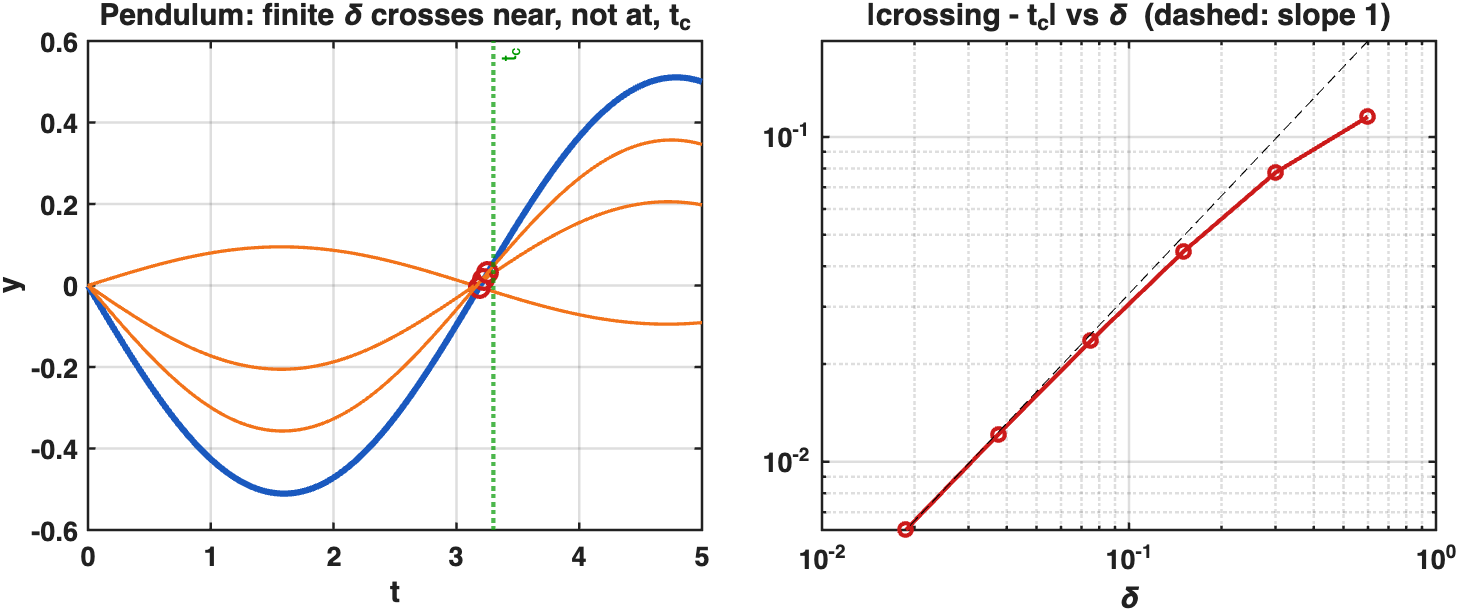
\includegraphics[width=\textwidth]{figures/pendulum_limit.png}
\caption{The pendulum $F = y'^2/2 + \cos y$ on $[0,5]$. Left: neighbours with
$\delta = 0.6, 0.3, 0.15$ cross near, not at, $t_c = 3.3011$. Right: the crossing
error halves when $\delta$ halves (slope 1 on log--log axes).}
\label{fig:pend}
\end{figure}

% =======================================================================
\section{Guided experiments}

Open the explorer (\file{conjugate\_point\_explorer}) and work through these in
order. Each asks you to \emph{predict} first. The checkpoints are the values
\file{conjugate\_point\_study.m} computed and verified.

\begin{expt}{1: the oscillator, before and after $\pi$}
Preset \emph{Oscillator, b = 3}. Predict: $F = y'^2 - y^2$ gives $y'' = -y$, so
$h = \sin t$. Where are the conjugate points? Is $b = 3$ before or after the
first one? Read the verdict. Switch to \emph{Oscillator, b = 4} and compare.
\begin{chk}
$b = 3$: one extremal, $J = \cot 3 = -7.015253$, $\lambda_1 = +0.1933$, verdict
\emph{weak local minimiser}. $b = 4$: $y'(0) = 1/\sin 4 = -1.32134871$,
$J = \cot 4 = 0.863691$, $t_c = \pi$ to ten digits, $\lambda_1 = -0.7663$, every
neighbour crosses at $\pi$ for any $\delta$, verdict \emph{not a minimiser}.
\end{chk}
\end{expt}

\begin{expt}{2: two conjugate points}
Preset \emph{Oscillator, b = 7}. Predict how many negative modes the second
variation has, then look at the Morse line.
\begin{chk}
Zeros of $h$ at $\pi$ and $2\pi$ inside $(0,7)$; negative modes $= 2$;
$\lambda_1 = -1.5972$. Figure~\ref{fig:morse} shows why: one eigenvalue crosses
zero each time $b$ passes $k\pi$.
\end{chk}
\end{expt}

\begin{expt}{3: a finite nudge on a nonlinear problem}
Preset \emph{Pendulum}. There are two extremals; select the second. Compare the
first crossings of the four neighbours with $t_c$ in the readout, then press
\emph{Shrink} and watch them converge. Now select the first extremal: where is
its conjugate point?
\begin{chk}
Extremal 2: $y'(0) = -0.505173$, $J = 4.968943$, $t_c = 3.301088$. Crossing
errors at $\delta = 0.6, 0.3, 0.15, 0.075, 0.0375, 0.01875$:
$0.115, 0.078, 0.044, 0.024, 0.012, 0.0062$ (halving ratios rise to $1.97$:
first order). Extremal 1: $y'(0) = -1.834052$, $J = 3.690547$, first zero of $h$
at $6.636 > b$: a weak local minimiser, and the lower of the two costs.
\end{chk}
\end{expt}

\begin{expt}{4: two catenaries}
Preset \emph{Minimal surface}. $F = y\sqrt{1+y'^2}$ is the area (divided by $2\pi$)
of the surface made by spinning $y(t)$ about the $t$-axis. Two catenaries
$y = c\cosh(t/c)$ pass through the ends. Predict which is the minimiser. Check
all four views for both.
\begin{chk}
$c = 0.848338$ (shallow) and $0.235095$ (deep), from $c\cosh(1/2c) = 1$. Shallow:
$y'(a) = -0.624109$, $J = 0.953624$, no conjugate point, $\lambda_1 = +5.839$,
$\Delta J > 0$. Deep: $y'(a) = -4.134382$, $J = 1.089520$, $t_c = 0.15291144$,
$\lambda_1 = -2.366$, $\Delta J < 0$. The conjugate point agrees to eight digits
with Lindel\"of's classical construction --- the tangents to the catenary at $a$
and at $t_c$ meet the $t$-axis at the same point \cite{bliss} --- which uses no
Jacobi equation at all.
\end{chk}
\end{expt}

\begin{expt}{5: the fold}
Stay on the minimal surface and widen the gap symmetrically: set
$a = -L$, $b = L$ with $L = 0.6$, $0.65$, $0.66$, then $0.67$. Watch the deep
catenary's $t_c$ approach $b$, the two roots of $r(p)$ approach each other, and
then disappear.
\begin{chk}
Two catenaries exist only for $L < L^* = 0.662743$ (where $x\tanh x = 1$,
$L^* = x/\cosh x$). The gap $b - t_c$ on the deep one: $0.347, 0.307, 0.180, 0.092$
at $L = 0.5, 0.6, 0.65, 0.66$. At $L = 0.67$ there is no extremal at all: the
soap film breaks. At the fold, $b$ is conjugate to $a$ and $r'(p) = h(b) = 0$ ---
the two extremals merge there.
\end{chk}
\end{expt}

\begin{expt}{6: never a conjugate point}
Preset $F = y'^2 + y^2$, then \emph{Arc length}. Predict $h$ for each.
\begin{chk}
$y'^2 + y^2$: $h = \sinh t$, never zero; arc length: $h = t - a$, never zero.
Both are minimisers on every interval.
\end{chk}
\end{expt}

\begin{expt}{7: your own Lagrangian}
Choose \emph{Custom}. Type $F = $ \file{yp\^{}2 - 4*y\^{}2} on $[0, 3]$ with
$y(0) = 0$, $y(3) = 1$. Predict $t_c$ before pressing \emph{Solve}. Then try
\file{y\^{}2 - yp\^{}2}: what does the Legendre line say, and why is the Morse
count marked not applicable?
\begin{chk}
$y'' = -4y$, $h = \tfrac12\sin 2t$, $t_c = \pi/2 = 1.570796$, not a minimiser.
For $F = y^2 - y'^2$, $P = -2 < 0$: Legendre's necessary condition fails, so the
extremal is not a minimiser whatever the Jacobi field does; fast wiggles make
$\delta^2 J$ unboundedly negative, so every fine mode is negative.
\end{chk}
\end{expt}

% =======================================================================
\section{How the code is organised, and how it is checked}

\begin{center}\small
\begin{tabular}{@{}ll@{}}
\toprule
file & role \\
\midrule
\file{cov\_problem.m} & text $F$ $\to$ $g$, $g_y$, $g_{y'}$, $P$, $R$, $Q_0$ (symbolic) \\
\file{cov\_shoot.m} & extremal + Jacobi field from $(a, y_a)$ with slope $p$; zeros of $h$ \\
\file{cov\_extremals.m} & scan $r(p)$, refine sign changes: every extremal in the range \\
\file{cov\_perturbed.m} & the neighbour with slope $p + \delta$ and its crossings \\
\file{cov\_second\_variation.m} & finite-element $\delta^2 J$: eigenvalues, $\eta^*$, exact $\Delta J$ \\
\file{cov\_functional.m} & $J[y_0 + \eta]$ by 4-point Gauss quadrature \\
\file{conjugate\_point\_explorer.m} & the GUI (programmatic, with a handle API for tests) \\
\file{conjugate\_point\_study.m} & every fact in this guide, computed and checked \\
\file{run\_conjugate\_tests.m} & the suite, one exit code \\
\bottomrule
\end{tabular}
\end{center}

Nothing is checked against a copy of itself. The oracles are closed forms (the
oscillator's $\sin t$, $\cot b$, $k\pi$ and $2((k\pi/b)^2 - 1)$; the catenary's
$c\cosh(1/2c) = 1$ and its area), a geometric construction (Lindel\"of's
tangents), and a second instrument (the Morse count against the Jacobi zeros,
and $r'(p)$ by finite differences against $h(b)$). A mutation test corrupts the
Jacobi equation, the Legendre coefficient and the integrand in turn, and requires
the check aimed at each corruption to fail --- and only that one.

% =======================================================================
\section{The same idea in the orbit-transfer library}

The conjugate-point test in the costate library
(\file{orbit\_transfer/costate\_common/ms\_conjugate\_test.m},
\file{conj\_spectrum.m}) is this construction in six dimensions. The ``initial
slope'' is the initial costate $\lambda(0)$; the Jacobi field is the block of the
state-transition matrix $\partial(r,v)(t)/\partial\lambda(0)$, restricted by a
projection $P$ to the costate directions that keep the problem normalised; and
the conjugate point is where that block, augmented by the flow direction $f_{rv}$
to account for the free final time, loses rank:
$\det[\Phi_{rv}P,\; f_{rv}] = 0$ --- the multidimensional $h(c) = 0$. A family of
neighbouring min-time trajectories, all leaving the same departure state with
slightly different costates, refocusing before arrival: the same picture as the
orange curves in Figure~\ref{fig:explorer}.

% =======================================================================
\begin{thebibliography}{9}
\bibitem{gelfand} I.~M. Gelfand and S.~V. Fomin, \emph{Calculus of Variations},
Prentice-Hall, 1963, Ch.~5 (the second variation; Jacobi's equation; conjugate
points; sufficient conditions for a weak extremum).
\bibitem{liberzon} D.~Liberzon, \emph{Calculus of Variations and Optimal Control
Theory: A Concise Introduction}, Princeton University Press, 2012, Ch.~2.
\bibitem{milnor} J.~Milnor, \emph{Morse Theory}, Annals of Mathematics Studies 51,
Princeton University Press, 1963, Part~III (the index theorem).
\bibitem{bliss} G.~A. Bliss, \emph{Calculus of Variations}, Carus Mathematical
Monographs No.~1, Mathematical Association of America, 1925 (the surface of
revolution of minimum area).
\end{thebibliography}

\end{document}
